\documentclass[11pt, oneside]{article}   	% use "amsart" instead of "article" for AMSLaTeX format
\usepackage{geometry}                		% See geometry.pdf to learn the layout options. There are lots.
\geometry{letterpaper}                   		% ... or a4paper or a5paper or ... 
%\geometry{landscape}                		% Activate for rotated page geometry
%\usepackage[parfill]{parskip}    		% Activate to begin paragraphs with an empty line rather than an indent
\usepackage{graphicx}				% Use pdf, png, jpg, or eps§ with pdflatex; use eps in DVI mode
								% TeX will automatically convert eps --> pdf in pdflatex		
\usepackage{amssymb}
\usepackage{amsmath,amssymb,amsthm,amsfonts,hyperref,fancyhdr,graphicx,subfig,bbm,multirow,array,longtable}

%SetFonts

%SetFonts

\title{Deep Learning}
\author{Bastien BRIER\\ bastien.brier@student.ecp.fr}
\date{March 5, 2017}				% Activate to display a given date or no date

\begin{document}
\maketitle
\vspace{-10pt}
\begin{center}
{\LARGE \bf Assignment 3}\\
\vspace{10pt}
\end{center}

\section{Training Neural Networks}
\vspace{4pt}

\subsection{Understanding the code}
\vspace{4pt}
We found the symbols associated to the variables slide 142 in the 4th presentation.\\
 - \texttt{d\_output\_d\_activation} = $ \frac{\partial \hat{y}_{c}}{\partial b_{k}} $\\
 - \texttt{d\_loss\_d\_activation} = $ \frac{\partial L}{\partial b_{k}} $\\
 - \texttt{d\_loss\_d\_output} = $ \frac{\partial L}{\partial \hat{y}_{c}} $\\
\newline
We are here applying the L2-regularization cost on the weights to modify them accordingly during the back-propagation process, a larger regularization means that we decrease the importance of each neuron on the output. We start from 2 because we added a constant vector and we do not want to regularize it.\\
\newline
We are here computing the error term for each output, which means how much a node is responsible for the error. In the case of one hidden layer, it is first computed between the output and layer, and then layer and input. This corresponds to the slide 149 of the 4th presentation.

\subsection{Extension: Using Softmax}
\vspace{4pt}
In the provided code, we modified the objective function from the sigmoid to the softmax. For this, we implemented the function softmax.m and modified parts of the code nnet.m that are indicated by doSoftMax. Then, if doSoftMax is set to true, the softmax is used in the neural network.

\subsection{Extension: Using ReLUs}
\vspace{4pt}
We modified the code by implementing a new activation function, a rectified linear unit (ReLU). We implemented the functions ReLU.m and reluGradient.m and also modified parts of the code nnet.m that are indicated by doReLU. Similarly, is this is set to true, the ReLU activation is used.

\subsection{Experiment: Cross-validate over regularization cost and number of intermediate neurons}
\vspace{4pt}
Thanks to the template provided, we implemented a 10-fold cross-validation on the regularization cost $\lambda$ and the number of neurons N for three different models : Softmax, ReLU and Softmax-ReLU.\\
We obtained really satisfactory results for the three models. The graphs corresponds to the results for the different parameters: the ordinate is the regularization cost : the lower, the higher the regularization. The abscissa is the number of neurons : from left to right correspond to 5, 10, 20, 50 and 100 neurons. For a better comprehension, a darker and bluer color corresponds to a lower error.\\
	\begin{figure}[h]
		\raggedleft
		\caption{Cross-validation error for softmax (left), relu (middle) and softmax-relu (right) combinations.}
		\begin{tabular}[h]{lll}
			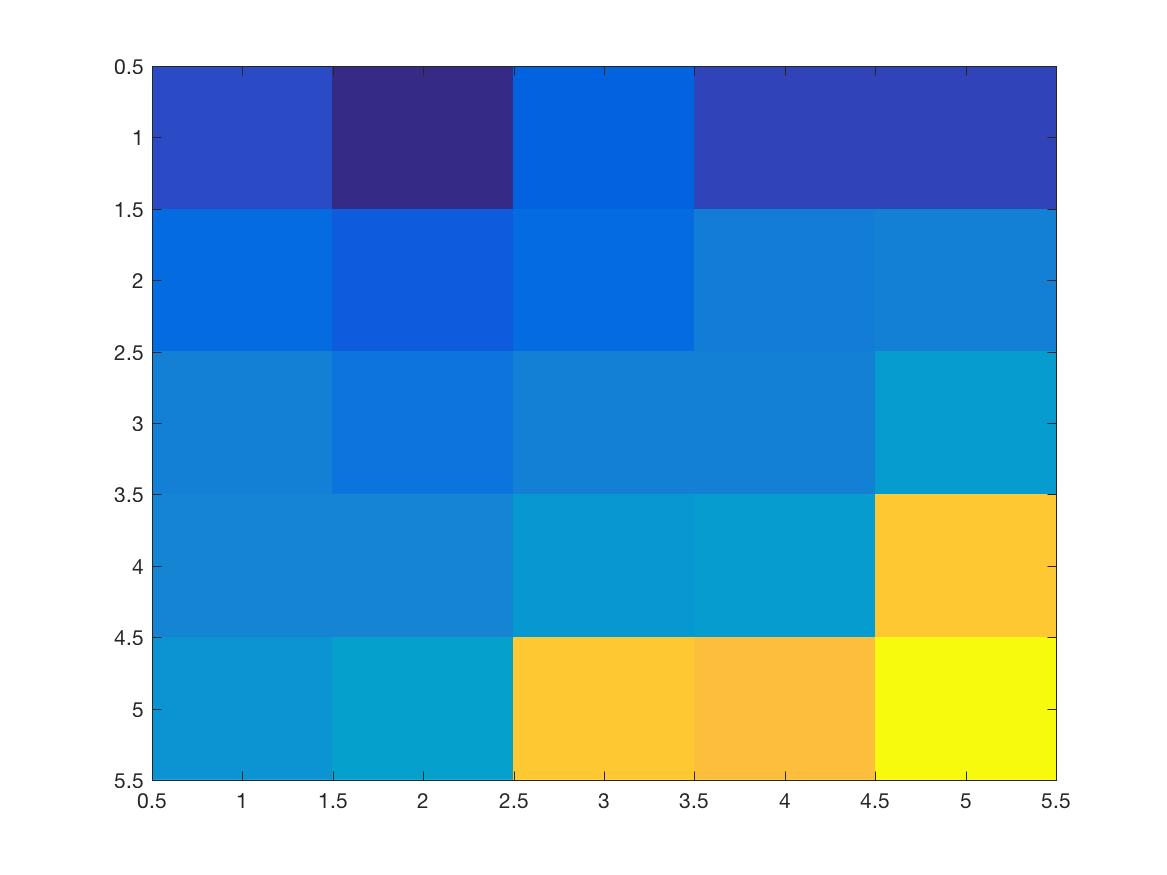
\includegraphics[width=5cm]{/Users/bastienbrier/Pictures/CV_softmax.jpg}
			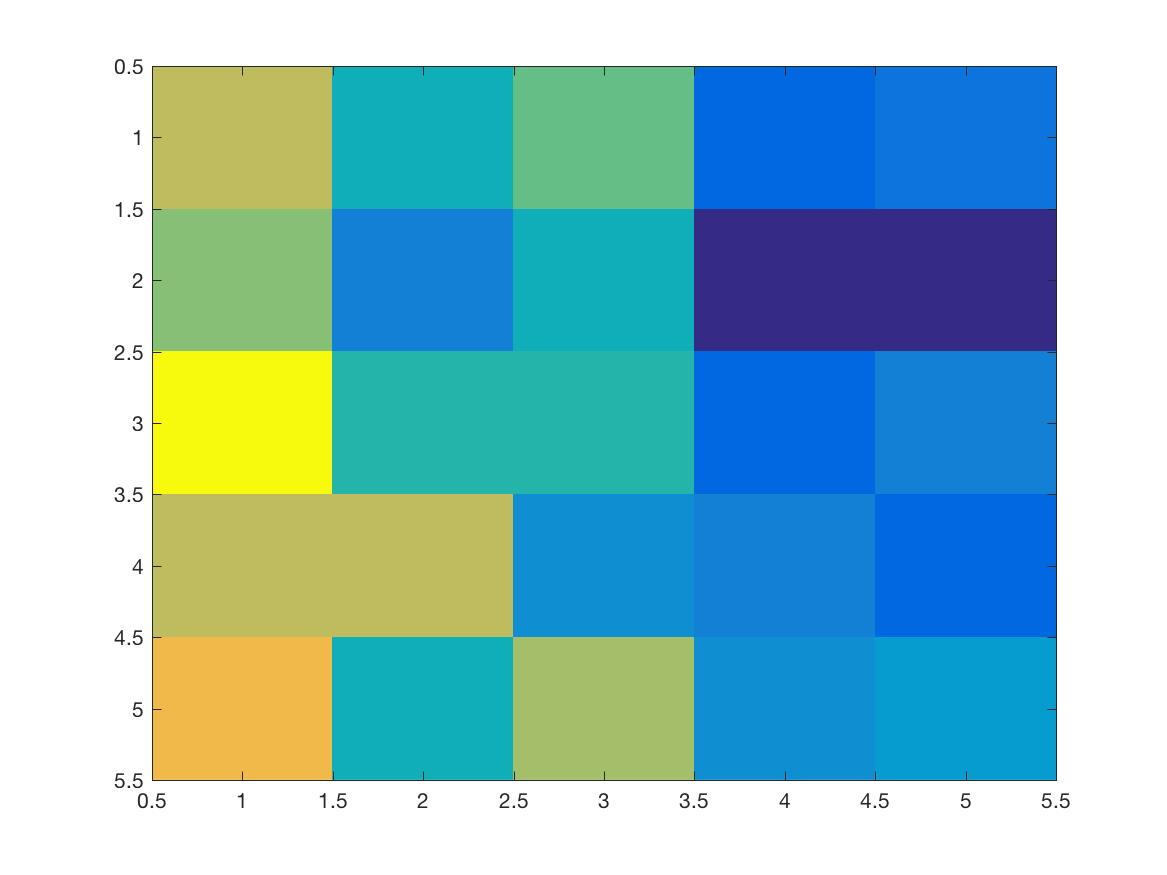
\includegraphics[width=5cm]{/Users/bastienbrier/Pictures/CV_relu.jpg}
			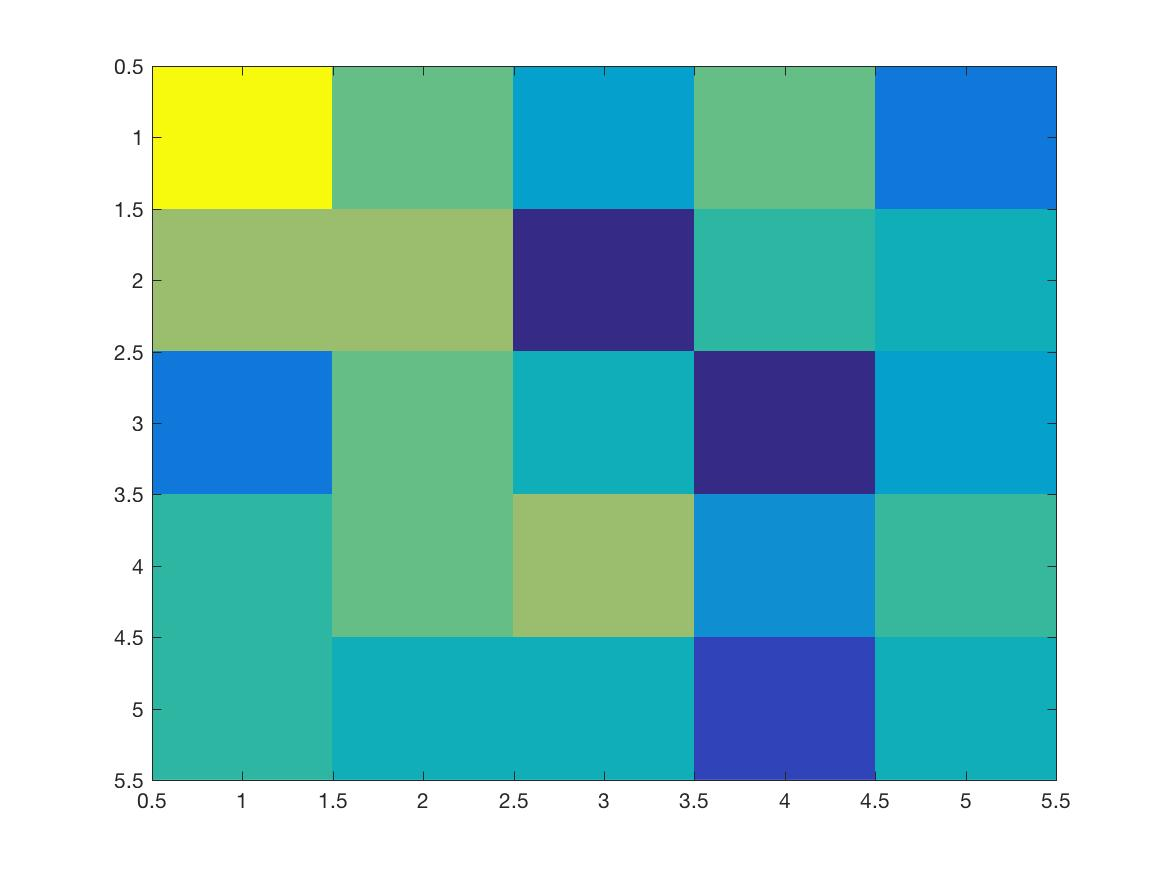
\includegraphics[width=5cm]{/Users/bastienbrier/Pictures/CV_softmax-relu.jpg}
		\end{tabular}
	\end{figure}
 
\end{document}  